\documentclass[a4paper, 10pt]{article}

\usepackage[english]{babel}
\usepackage[T1]{fontenc}
\usepackage[utf8]{inputenc}
\usepackage{textcomp}
\setlength{\marginparwidth}{2cm}

\usepackage{comment}
\usepackage{todonotes}

\usepackage{amsmath}
\usepackage{amssymb}
\usepackage{bm}

\usepackage{enumitem}
\usepackage{array}
\setlength\extrarowheight{5pt}

\usepackage{xcolor}
\usepackage{graphicx}
\graphicspath{ {./img/} }

\usepackage{hyperref}
\usepackage{listings}
\usepackage{color}
\definecolor{dkgreen}{rgb}{0,0.6,0}
\definecolor{gray}{rgb}{0.5,0.5,0.5}
\definecolor{mauve}{rgb}{0.58,0,0.82}
\lstset{frame=tb,
    language=Python,
    aboveskip=3mm,
    belowskip=3mm,
    showstringspaces=false,
    columns=flexible,
    basicstyle={\small\ttfamily},
    numbers=none,
    numberstyle=\tiny\color{gray},
    keywordstyle=\color{blue},
    commentstyle=\color{dkgreen},
    stringstyle=\color{mauve},
    breaklines=true,
    breakatwhitespace=true,
    tabsize=3
}

\title{Homework Assignment N°4}
\author{BML36\\Thibault Douzon\\Rajavarman Mathivanan}
\date{October 3rd, 2018}

\begin{document}
\maketitle

\pagebreak

\tableofcontents

\pagebreak
\section{Exercise 1: NN 1-D output}
\subsection{Part a}
The neural network described in this exercise could be represented like this.
\begin{center}
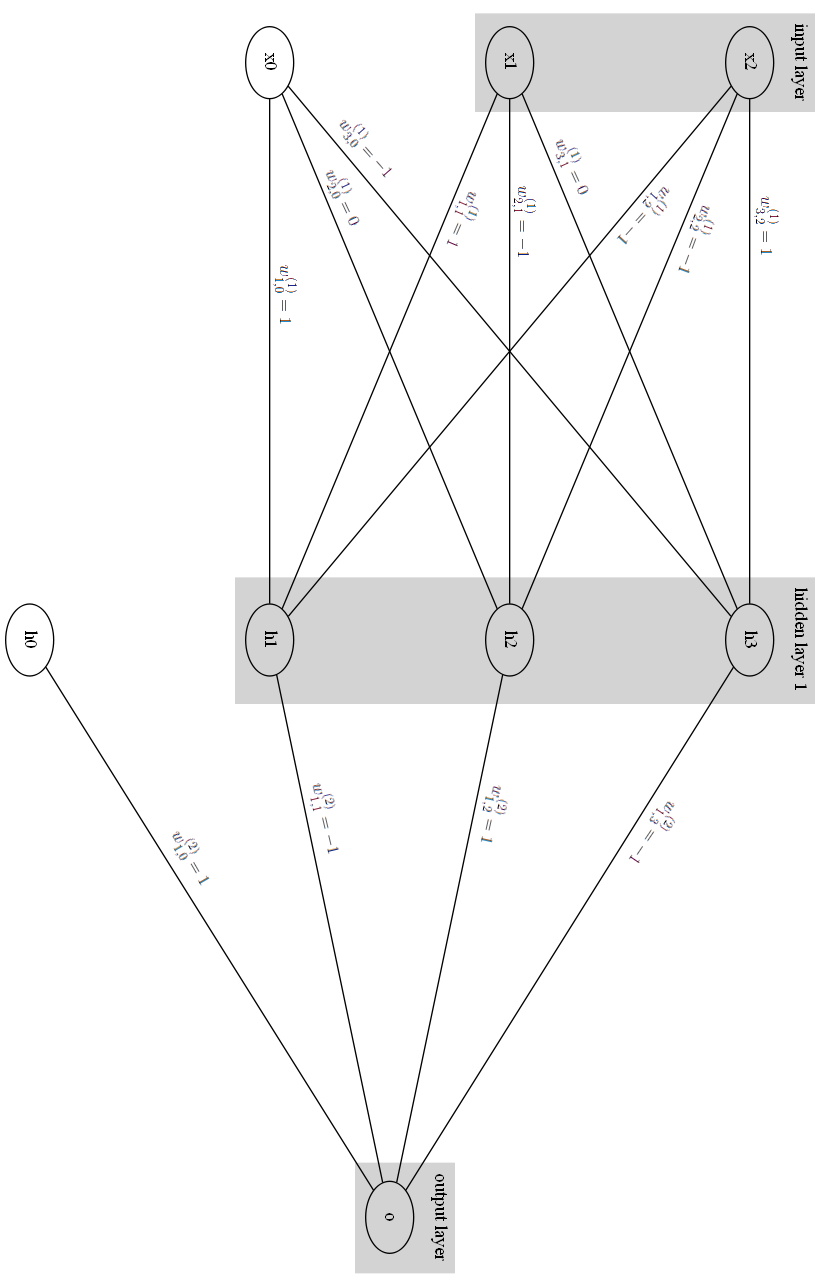
\includegraphics[scale=0.5]{ex1_graph_export}
\end{center}
It is structured in 3 parts: the input layer first (denoted $x1$, $x2$), then the hidden layer
(denoted $h1$, $h2$ and $h3$) and then the output layer (denoted $o$).
\\
Nodes with indice 0 represent the bias introducted into the model.
\\ 
Each arc carries the value of the weight (denoted $w_{k,j}^{(l)}$ where $l$ is the layer, $k$ is the destination node
and $j$ is the origin node which lies in the layer $l-1$).

To compute the output of the neural network, we need to propagate
through the network the values of the input. Hidden and output layer applies a sigmoïd activation function.
\\
Thus we can first compute every $a_k^{(1)}$, the signal recieved by each node in the hidden layer.
It is easier to make this computation under matrix representation, let's introduce the input vector $X$ and
the weights of the first layer $W^{(1)}$:
$$
X = [a_i^{(0)}] = [x_i] =\begin{bmatrix}
    1\\
    1\\
    1
\end{bmatrix}
$$
$$
W^{(1)} = [w_{j,i}^{(1)}] =  \begin{bmatrix}
    1 & 0 & -1\\
    1 & -1 & 0\\
    -1 & -1 & 1
\end{bmatrix}
$$
The signal recieved by the hidden layer is given by the following formula:
$$
H_{j\ne0} = [a_j^{(1)}]_{j\ne0} = X^\top W^{(1)} = \begin{bmatrix}
    1\\
    -2\\
    0
\end{bmatrix}
$$
Before repeating the same procedure, we need to apply the activation function
to each recieved signal and then concatenate the bias.
\\
The hidden layer uses the sigmoïd function as activation:
$$
\sigma(H_{j\ne0}) = [\sigma(a_j{(1)})] = \begin{bmatrix}
    \sigma(1)\\
    \sigma(-2)\\
    \sigma(0)
\end{bmatrix}
\approx \begin{bmatrix}
        0.731\\
        0.119\\
        0.5
\end{bmatrix}
$$
Now we can concatenate the bias at the beginning with a fixed value of 1:
$$
H_{out} \approx \begin{bmatrix}
    1\\
    0.731\\
    0.119\\
    0.5
\end{bmatrix}
$$
The vector $H_{out}$ is the signed emitted by the hidden layer.
\\
We can now repeat the same procedure with the second layer with $H_{out}$ as input and 
use the weights of the output layer.
\\
The weights of the second layer are the following:
$$
W^{(2)} = [w_{k,j}^{(2)}] = \begin{bmatrix}
    1\\
    -1\\
    1\\
    -1
\end{bmatrix}
$$
And we can compute the signal recieved by the output layer:
$$
O = [a_k^{(2)}] = {H_{out}}^\top W^{(2)} \approx \begin{bmatrix}
    -0.112
\end{bmatrix}
$$
We just have to apply the activation function of the output layer to get the output of the network:
$$
y(x) = \sigma(O) \approx \sigma(-0.112) \approx 0.472
$$
This is the final result of our network for the provided input.

\subsection{Part b}

Partial differentiation the error function with respect to activation function will give us $\delta$.
We use the following error formula:
$$
E_n=- (t_n\ln (y_n)  +(1-t_n)\ln (1-y_n))
$$
Where $y_n=\sigma(a_1^{(2)})$ is the output of the network for an input $x_n$.
\\
Finding gradient of error function with respect to activation function
$$
\delta _{1}^{(2)}= \frac{\partial E }{\partial y_{n}}\frac{\partial y_{n}}{\partial a_1^{(2)}}
$$
$$
\delta _{1}^{(2)}=  -\frac{\partial (t_n\ln (y_n)  +(1-t_n)\ln (1-y_n))}{\partial \sigma(a_1^{(2)})}\frac{\partial \sigma(a_1^{(2)})}{\partial a_1^{(2)}}
$$
$$
\delta _{1}^{(2)}= -\left[\frac{t_n}{y_n}-\frac{1-t_n}{1-y_n}\right]\cdot\sigma(a_1^{(2)})(1-\sigma(a_1^{(2)}))
$$
Regroup the fractions together and replace $\sigma(a_1^{(2)})$ by $y_n$:
$$
\delta _{1}^{(2)}= -\left[\frac{(1-y_n)t_n -(1-t_n)y_n}{(1-y_n)y_n}\right]y_n(1-y_n) 
$$
Simplify the $y_n(1-y_n)$ terms:
$$
\delta _{1}^{(2)}= -[(1-y_n)t_n - (1-t_n)y_n]
$$
And now expand and simplify again to obtain the final expression for $\delta$:
$$
\delta _{1}^{(2)}= y_n-t_n
$$
We can now compute the value of $\delta$ for the given input and target:
$$
\delta _{1}^{(2)}= y_n-t_n \approx 0.472 - 1 \approx -0.528
$$

\subsection{Part c}
New weights can be calculated by applying the below formula
$$
w^{[\tau +1]}=w^{[\tau]}-\eta\nabla_w E_n
$$
Apply chain rule for $\nabla_{w_{1,2}^{(2)}}E_n$
$$
\nabla_{w_{1,2}^{(2)}}E_n=\frac{\partial E_n}{\partial {w_{1,2}^{2}}}=\frac{\partial E_n}{\partial y_n}\cdot\frac{\partial y_n}{\partial a_1^{(2)}}\cdot\frac{\partial a_1^{(2)}}{\partial {w_{1,2}^{(2)}}}
$$
$$
\nabla_{w_{1,2}^{(2)}}E_n= \delta_1^{(2)} \cdot \frac{\partial a_1^{(2)}}{\partial w_{1,2}^{(2)}}
$$
$$
a_1^{(2)}=(w_{1,0}^{(2)})+\sigma(a_1^{(1)})w_{1,1}^{(2)}+\sigma(a_2^{(1)})w_{1,2}^{(2)}+\sigma(a_3^{(1)})w_{1,3}^{(2)}
$$
where $a_i^{(l)}$ is the activation of the neuron $i$ in layer $l$.
$$
\nabla_{w_{1,2}^{2}}E_n=\delta_1^{(2)}\cdot \sigma(a_2^{(1)}) \approx (-0.528)\cdot0.5\approx -0.264
$$
Hence the updated weight is
$$
w_{1,2}^{(2)[2]}=w_{1,2}^{(2)[1]} - \eta \nabla_{w_{1,2}^{2}}E_n \approx 1-0.7\cdot(-0.264) \approx 1.185
$$
\subsection{Part d}
The formula to compute $\delta$ is still the following one:
$$
\delta_i^{(l)} = \frac{\partial E_n}{\partial a_i^{(l)}}
$$
Thus in our case, because the output is 1 dimensional:
$$
\delta_1^{(1)} = \frac{\partial E_n}{\partial a_1^{(1)}} = \frac{\partial E_n}{\partial a_1^{(2)}}\frac{\partial a_1^{(2)}}{\partial a_1^{(1)}}
$$
We can replace $\frac{\partial E_n}{\partial a_1^{(2)}}$ with $\delta_1^{(2)}$:
$$
\delta_1^{(1)} = \delta_1^{(2)} \frac{\partial a_1^{(2)}}{\partial a_1^{(1)}}
$$
And because 
$$
a_1^{(2)}=(w_{1,0}^{(2)})+\sigma(a_1^{(1)})w_{1,1}^{(2)}+\sigma(a_2^{(1)})w_{1,2}^{(2)}+\sigma(a_3^{(1)})w_{1,3}^{(2)}
$$
We deduce that $\frac{\partial a_1^{(2)}}{\partial a_1^{(1)}} = w_{1,1}^{(2)}\sigma^\prime(a_1^{(1)})$
\\
And finally we obtain the following formula:
$$
\delta_1^{(1)} = \sigma^\prime(a_1^{(1)}) w_{1,1}^{(2)}\delta_1^{(2)} 
$$
Using the fact that $\sigma^\prime(x) = \sigma(x)(1-\sigma(x))$ we can rewrite it:
$$
\delta_1^{(1)} = \sigma(a_1^{(1)})(1-\sigma(a_1^{(1)}))w_{1,1}^{(2)}\delta_1^{(2)} 
$$
$$
\delta_1^{(1)} \approx 0.731\cdot(1-0.731)\times (-1)\cdot(-0.528) \approx 0.104
$$
During the first backpropagation, the value of $\delta_1^{(1)}$ is roughly $0.104$

\subsection{Part e}
calculation of new weights formula
$$
w^{[\tau+1]}=w^{[\tau]}-\eta\nabla_w E_n
$$
Given $\eta=0.7$, substitute the corresponding old weights and $\nabla_{w_{1,i}^{(1)}}E_n=\delta_1^{(1)}\cdot x_i$
for the bias:
$$
w_{1,0}^{(1)[2]}= w_{1,0}^{(1)[1]}-\eta\nabla_{w_{1,0}^{(1)}}E_n = w_{1,0}^{(1)[1]}-\eta\delta_1^{(1)}x_0
$$
$$
w_{1,0}^{(1)[2]}\approx 1-0.7\cdot0.104\cdot1 \approx0.927
$$
For the first input:
$$
w_{1,1}^{(1)[2]}= w_{1,1}^{(1)[1]}-\eta\nabla_{w_{1,1}^{(1)}}E_n = w_{1,1}^{(1)[1]}-\eta\delta_1^{(1)}x_1
$$
$$
w_{1,1}^{(1)[2]}\approx 1-0.7\cdot0.104\cdot1 \approx0.927
$$
For the second input:
$$
w_{1,2}^{(1)[2]}= w_{1,2}^{(1)[1]}-\eta\nabla_{w_{1,2}^{(1)}}E_n = w_{1,2}^{(1)[1]}-\eta\delta_1^{(1)}x_2
$$
$$
w_{1,2}^{(1)[2]}\approx (-1)-0.7\cdot0.104\cdot1 \approx -1.073
$$

\section{Exercise 2: NN 2-D output}
\subsection{Part a}
The neural network described in this exercise could be represented like this.
\begin{center}
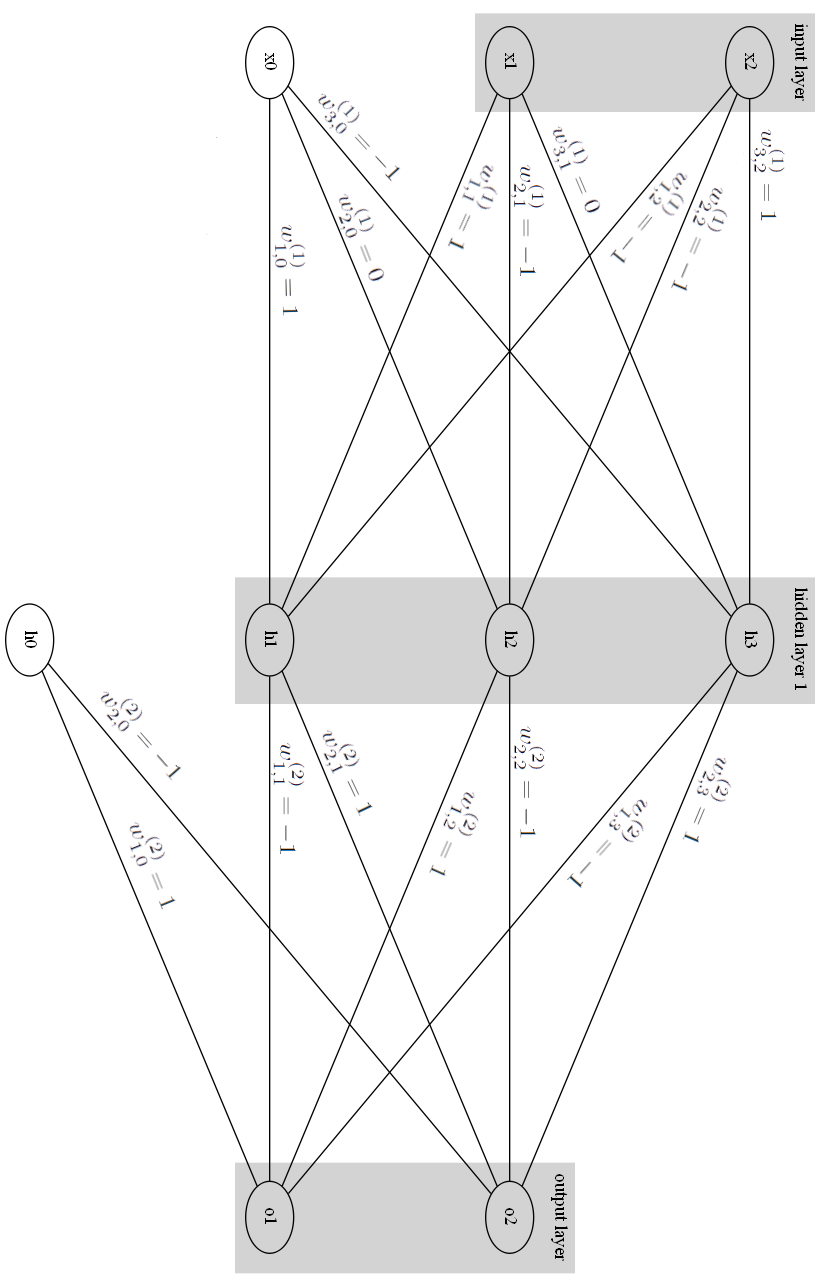
\includegraphics[scale=0.5]{ex2_graph_export}
\end{center}
It is structured in 3 parts: the input layer first (denoted $x1$, $x2$), then the hidden layer
(denoted $h1$, $h2$ and $h3$) and then the output layer (denoted $o1$ and $o2$).
\\
Nodes with indice 0 represent the bias introducted into the model.
\\ 
Each arc carries the value of the weight (denoted $w_{k,j}^{(l)}$ where $l$ is the layer, $k$ is the destination node
and $j$ is the origin node which lies in the layer $l-1$).

To compute the output of the neural network, we need to propagate
through the network the values of the input. Hidden layer applies a sigmoïd activation function
and output neurons have a linear activation function (identity function).
\\
Thus we can first compute every $a_k^{(1)}$, the signal recieved by each node in the hidden layer.
It is easier to make this computation under matrix representation, let's introduce the input vector $X$ and
the weights of the first layer $W^{(1)}$:
$$
X = [a_i^{(0)}] = [x_i] =\begin{bmatrix}
    1\\
    1\\
    1
\end{bmatrix}
$$
$$
W^{(1)} = [w_{j,i}^{(1)}] =  \begin{bmatrix}
    1 & 0 & -1\\
    1 & -1 & 0\\
    -1 & -1 & 1
\end{bmatrix}
$$
The signal recieved by the hidden layer is given by the following formula:
$$
H_{j\ne0}^\top = [a_j^{(1)}]_{j\ne0} = X^\top W^{(1)} = \begin{bmatrix}
    1\\
    -2\\
    0
\end{bmatrix}
$$
Before repeating the same procedure, we need to apply the activation function
to each recieved signal and then concatenate the bias.
\\
The hidden layer uses the sigmoïd function as activation:
$$
\sigma(H_{j\ne0}) = [\sigma(a_j{(1)})] = \begin{bmatrix}
    \sigma(1)\\
    \sigma(-2)\\
    \sigma(0)
\end{bmatrix}
\approx \begin{bmatrix}
        0.731\\
        0.119\\
        0.5
\end{bmatrix}
$$
Now we can concatenate the bias at the beginning with a fixed value of 1:
$$
H_{out} \approx \begin{bmatrix}
    1\\
    0.731\\
    0.119\\
    0.5
\end{bmatrix}
$$
The vector $H_{out}$ is the signed emitted by the hidden layer.
\\
We can now repeat the same procedure with the second layer with $H_{out}$ as input and 
use the weights of the output layer.
\\
The weights of the second layer are the following:
$$
W^{(2)} = [w_{k,j}^{(2)}] = \begin{bmatrix}
    1 & -1\\
    -1 & 1\\
    1 & -1\\
    -1 & 1
\end{bmatrix}
$$
And we can compute the signal recieved by the output layer:
$$
O^\top = [a_k^{(2)}] = {H_{out}}^\top W^{(2)} \approx \begin{bmatrix}
    -0.112\\
    0.112
\end{bmatrix}
$$
This is the output of our neural network as the activation
fonction of the output neuron is the identity function.

\subsection{Part b}
The formula to compute $\delta_i^{(l)}$ is the following:
$$
\delta_i^{(l)} = \frac{\partial E_n}{\partial a_i^{(l)}}
$$
Where $l$ is the layer and $i$ is the index of the neuron.
\\
But to compute the value of this expression for different values of $l$ and $i$,
we need to know the expression of $E_n$ first. $E_n$ is the error of the network
on the data sample number $n$. It is defined as follows:
$$
E_n(w) = \frac{1}{2} \sum_{k=1}^D ( y_k(x_n,w)-t_{n,k})^2
$$
Where $N$ is the number of output neurons (in our case 2), $x_n$ the input data and 
$t_n$ the target related to $x_n$, $w$ the current weigths of the neural network and 
$y_k$ the function that computes the $k^\text{th}$ coordinate of the NN's prediction based on the input data.
\\
In our case, we can rewrite this expression to this:
$$
E_n(w) = \frac{1}{2} \sum_{k=1}^2( y_k(x_n, w)-t_{n,k})^2
$$
And because the activation function of the output layer is the identity function,
we also have the following equation:
$$
y_k(x_n,w) = h(a_k^{(2)}) = a_k^{(2)}
$$
The analytical expressions of $\delta_1^{(2)}$ and $\delta_2^{(2)}$ directly follows:
$$
\delta_i^{(2)} = \frac{\partial E_n}{\partial a_i^{(2)}} = \frac{1}{2}\frac{\partial  \sum_{k=1}^2( a_k^{(2)}-t_{n,k})^2}{\partial a_i^{(2)}} = a_i^{(2)} - t_{n,i}
$$
We finally get the following numerical values:
$$
\delta_1^{(2)} = a_1^{(2)} - t_{n,1} = -0.112 - 1 = -1.112
$$
$$
\delta_2^{(2)} = a_2^{(2)} - t_{n,2} = 0.112 - (-1) = 1.112
$$

\subsection{Part c}
The formula to update a weight is the same as in previous models:
$$
w^{[\tau +1]} = w^{[\tau]} - \eta \frac{\partial E_n}{\partial w}(w^{[\tau]})
$$
We can use it to compute the new value of weight $w_{2,1}^{(2)}$ 
\\
First we will focus on computing $\frac{\partial E_n}{\partial w_{2,1}^{(2)}}$:
$$
\frac{\partial E_n}{\partial w_{2,1}^{(2)}}(w) = \frac{\partial E_n}{\partial a_2^{(2)}} \cdot \frac{\partial a_2^{(2)}}{\partial w_{2,1}^{(2)}}(w)
$$
$$
\frac{\partial E_n}{\partial w_{2,1}^{(2)}}(w) = \delta_2^{(2)} \cdot \frac{\partial a_2^{(2)}}{\partial w_{2,1}^{(2)}}(w) 
$$
From our previous computation in part a, we know the formula for $a_2^{(2)}$:
$$
a_2^{(2)} = \sum_{i=1}^3 w_{2,i}^{(2)}\sigma(a_i^{(1)}) + w_{(2,0)}^{(2)}
$$
Hence we deduce:
$$
\frac{\partial a_2^{(2)}}{\partial w_{2,1}^{(2)}}(w) = \sigma(a_1^{(1)}) \approx 0.731
$$
And finally we get:
$$
\frac{\partial E_n}{\partial w_{2,1}^{(2)}}(w) = \delta_2^{(2)} \cdot \frac{\partial a_2^{(2)}}{\partial w_{2,1}^{(2)}}(w) \approx 1.112 \times 0.731 \approx 0.813 
$$
We can now apply the formula to update the weight for $w_{2,1}^{(2)}$:
$$
w_{2,1}^{(2)[2]} = w_{2,1}^{(2)[1]} - \eta \frac{\partial E_n}{\partial w_{2,1}^{(2)}}(w_{2,1}^{(2)[1]}) 
$$
$$
w_{2,1}^{(2)[2]} \approx 1 - 0.5 \times 0.813 \approx 0.594
$$
When applying backpropagation with learning rate of 0.5, the new value of $w_{2,1}^{(2)}$ is 0.594
\subsection{Part d}
The first formula from part b still stands:
$$
\delta_i^{(l)} = \frac{\partial E_n}{\partial a_i^{(l)}} 
$$
Now because $a_2^{(1)}$ takes part in every output node, we need to sum over all contributions to the output nodes.
Moreover, because the hidden layer does not use the identity function as activation, we need to take into account the contribution
of the activation funtion. This means we need to use the following formula from the lecture:
$$
\delta_i^{(l)} = \sum_k \frac{\partial E_n}{\partial a_k^{(l+1)}}\frac{\partial a_k^{(l+1)}}{\partial a_i^{(l)}}
$$
And we can rewrite it like in the lecture:
$$
\delta_i^{(l)} = h^\prime(a_i^{(l)})\sum_k w_{k,i}^{(l+1)}\delta_k^{(l+1)} 
$$
Which gives in our case:
$$
\delta_2^{(1)} = \sigma^\prime(a_2^{(1)})\sum_{k=1}^2 w_{k,2}^{(2)}\delta_k^{(2)} 
$$
Using the fact that $\sigma^\prime(x) = \sigma(x)(1-\sigma(x))$ we can rewrite it:
$$
\delta_2^{(1)} = \sigma(a_2^{(1)})(1-\sigma(a_2^{(1)}))\sum_{k=1}^2 w_{k,2}^{(2)}\delta_k^{(2)} 
$$
$$
\delta_2^{(1)} \approx 0.119\cdot(1-0.119)\times [1\cdot(-1.112)+(-1)\cdot1.112] \approx -0.233
$$
During the first backpropagation, the value of $\delta_2^{(1)}$ is roughly $-0.233$
\subsection{Part e}
In this part we want to compute the weights of the neuron 2 of the hidden layer, $\forall k \in \{0,1,2\}, w_{2,k}^{(1)}$ in a more precise way 
\\
This is very similar to part c, we need to update some weights so we will use the same formula:
$$
w^{[\tau +1]} = w^{[\tau]} - \eta \frac{\partial E_n}{\partial w}(w^{[\tau]})
$$
Where we can use the following formula to compute the gradient:
$$
\frac{\partial E_n}{\partial w_{2,k}^{(1)}}(w) = \delta_2^{(1)} \cdot \frac{\partial a_2^{(1)}}{\partial w_{2,k}^{(1)}}(w),  \forall k\in\{0,1,2\} 
$$
And the term $\frac{\partial a_2^{(1)}}{\partial w_{2,k}^{(1)}}(w)$ can be simplified like this:
$$
\frac{\partial a_2^{(1)}}{\partial w_{2,k}^{(1)}}(w) = x_k, \forall k \in\{0,1,2\}
$$
Where $x_k$ is the $k^\text{th}$ coordinate of the input. To simplify the notation, it uses the convention that says $x_0=1$ to
include the bias inside the input vector.
\\
Now we are prepared to replace each term with its value for every weight wwe want to update:
$$
w_{2,k}^{(1)[\tau +1]} = w_{2,k}^{(1)[\tau]} - \eta \delta_2^{(1)}x_k, \forall k \in \{0,1,2\}
$$
For $w_{2,0}^{(1)}$:
$$
w_{2,0}^{(1)[2]} = w_{2,0}^{(1)[1]} - \eta \delta_2^{(1)}x_0
$$
$$
w_{2,0}^{(1)[2]} \approx 0 - 0.5\cdot(-0.233)\cdot1 \approx 0.117
$$
For $w_{2,1}^{(1)}$:
$$
w_{2,1}^{(1)[2]} = w_{2,1}^{(1)[1]} - \eta \delta_2^{(1)}x_1
$$
$$
w_{2,1}^{(1)[2]} \approx (-1) - 0.5\cdot(-0.233)\cdot1 \approx -0.884
$$
For $w_{2,2}^{(1)}$:
$$
w_{2,2}^{(1)[2]} = w_{2,2}^{(1)[1]} - \eta \delta_2^{(1)}x_2
$$
$$
w_{2,2}^{(1)[2]} \approx (-1) - 0.5\cdot(-0.233)\cdot1 \approx -0.884
$$
Those values are the new weights for neuron 2 in the hidden layer.

\section{Exercise 3: Weight sharing}
\subsection{Part a}
The base formula to update the value of a weight is the one we used in previous exercises:
$$
w^{[\tau +1]} = w^{[\tau]} - \eta \frac{\partial E_n}{\partial w}(w^{[\tau]})
$$
Our goal is now to figure out the formula for $\frac{\partial E_n}{\partial w_{1,2}^{(1)}}$ in term of $\delta$'s and inputs.
\\
The regular formula in most simple case is the following:
$$
\frac{\partial E_n}{\partial w_{j,i}^{(l)}}(w) = \delta_j^{(l)} \cdot \frac{\partial a_j^{(l)}}{\partial w_{j,i}^{(l)}}(w) 
$$
As $w_{1,2}^{(1)}$ appears multiple times in the network, we need to sum up on every hidden node where our weight appears its contribution in order to get the correct value.
We define $H_{j,i,l}$ to be the set of the node's indices our weight belongs to. It results the following:
$$
\frac{\partial E_n}{\partial w_{j,i}^{(l)}}(w) = \sum_{k\in H_{j,i,l}} \delta_k^{(l)} \cdot \frac{\partial a_k^{(l)}}{\partial w_{j,i}^{(l)}}(w) 
$$
Where, because we lay in the first layer, we can simplify $\frac{\partial a_k^{(l)}}{\partial w_{j,i}^{(l)}}(w)$ to $x_i$
We also need to define the set of input neuron's indices $I_{j,i,l}$ that wiil complete the information held in $H_{j,i,l}$. 
\\
Finally we get the following formula for the gradient for our weight:
$$
\frac{\partial E_n}{\partial w_{1,2}^{(1)}}(w) = \sum_{\substack{k\in H_{1,2,1}\\i\in I_{1,2,1}}} \delta_k^{(1)}x_i 
$$

In this exercise, we want to update $w_{1,2}^{(1)}$, thus $H_{1,2,1} = \{1,2\}$ and $I_{1,2,1} = \{2,3\}$.
Now we can complete our update formula by replcacing the gradiant by the expression we just found:
$$
w_{1,2}^{(1)[2]} = w_{1,2}^{(1)[1]} - \eta \sum_{\substack{k\in\{1,2\}\\i\in\{2,3\}}} \delta_k^{(1)}x_i
$$
Which develops to the following expression:
$$
w_{1,2}^{(1)[2]} = w_{1,2}^{(1)[1]} - \eta (\delta_1^{(1)}x_2 + \delta_2^{(1)}x_3)
$$
In the next question, we will use formulas similar to this one to update the weights.

\subsection{Part b}
First we need to compute the output of the network with input $x=[1,\ 1,\ 2,\ 3]^\top$ which already include the bias component.
\\
The weights of the first layer can be written like the following using matrices:
$$
W^{(1)} = \begin{bmatrix}
    1 & 0\\
    1 & \bm{0}\\
    -1 & 1\\
    \bm{0} & -1
\end{bmatrix} 
$$
In the previous matrix, some $0$ are bold because they cannot change their value as the weight does not exist.
No matter the update, those weights will remain zeros.
\\
We can now compute the activation of the hidden layer by multiplying inputs and weights:
$$
A^{(1)\top} = x^\top W^{(1)} = \begin{bmatrix}
    0 & -1
\end{bmatrix} 
$$
Now we apply the activation function on the hidden nodes:
$$
\sigma(A^{(1)})^\top = \begin{bmatrix}
    0.5 & 0.269
\end{bmatrix}
$$
And we concatenate with the bias:
$$
H_{out}^\top = \begin{bmatrix}
    1 & 0.5 & 0.269
\end{bmatrix}
$$
The activation of the output node is simply given by the multiplication of the out signal of the hidden layer by the weights of the 
output node. Those weights are the following:
$$
W^{(2)} = \begin{bmatrix}
    -1\\
    2\\
    -1
\end{bmatrix}
$$
And the ouput node activation follows:
$$
A^{(2)} = H_{out}^\top W^{(2)} = \begin{bmatrix}
    -0.269
\end{bmatrix}
$$
And because the activation function of the output node is linear, this result is the actual output of the neural network
on the given input.

Before trying to update the weights of the first neuron in the hidden layer, we will compute every $\delta$ we need.
We obviously need to compute $\delta_1^{(2)}$ because it takes part in $\delta$'s of both neuron in hidden layer.
We also need to compute $\delta_1^{(1)}$ because we want to update the weights of this neuron. We will also (and finally) need 
$\delta_2^{(1)}$ because some weights of the first neuron appears also in the weights of the second neuron.
\\
Let's start with $\delta_1^{(2)}$:
$$
\delta_1^{(2)} =  \frac{\partial E_n}{\partial a_1^{(2)}}
$$
With 
$$
E_n = \frac{1}{2} (y(x_n)-t_n)^2
$$
Where $y(x)$ denotes the output of the network for an input $x$ and $t$ is the target associated to $x$
But because the activation function of the output layer is the identity function, we have the followign identity:
$$
y(x) = a_1^{(2)}
$$
We deduce from the previous lines the expression of $\delta_1^{(2)}$:
$$
\delta_1^{(2)} = a_1^{(2)} - t_n
$$
And its value is approximately:
$$
\delta_1^{(2)} \approx (-0.269) - 0 = -0.269
$$
Now we need to compute both $\delta_1^{(1)}$ and $\delta_2^{(1)}$.
We will use the formula from the lectures:
$$
\delta_j^{(l)} = h^\prime(a_j^{(l)})\sum_k w_{k,j}^{(l+1)}\delta_k^{(l+1)} 
$$
Which simplifies in our case because the output is 1-dimension:
$$
\delta_j^{(1)} = h^\prime(a_j^{(1)})w_{1,j}^{(2)}\delta_1^{(2)} 
$$
In the hidden layer, the activation function is the sigmoïd, then we get our final formula:
$$
\delta_j^{(1)} = \sigma(a_j^{(1)})(1-\sigma(a_j^{(1)}))w_{1,j}^{(2)}\delta_1^{(2)} 
$$
We will use the previous formula for each neuron:
$$
\delta_1^{(1)} = \sigma(a_1^{(1)})(1-\sigma(a_1^{(1)}))w_{1,1}^{(2)}\delta_1^{(2)} 
$$
$$
\delta_1^{(1)} \approx \sigma(0)(1-\sigma(0))\cdot2\cdot(-0.269) \approx -0.135
$$
And now the second neuron:
$$
\delta_2^{(1)} = \sigma(a_2^{(1)})(1-\sigma(a_2^{(1)}))w_{1,2}^{(2)}\delta_2^{(2)} 
$$
$$
\delta_2^{(1)} \approx \sigma(-1)(1-\sigma(-1))\cdot(-1)\cdot(-0.269) \approx 0.053
$$

Now we will update each weight of the first neuron. The general formula to update a weight is the following one:
$$
w^{[\tau +1]} = w^{[\tau]} - \eta \frac{\partial E_n}{\partial w}(w^{[\tau]})
$$
We will start with the bias because its updating formula simplifies nicely as $\frac{\partial E_n}{\partial w_{1,0}^{(1)}}=\delta_1^{(1)}x_0$:
$$
w_{1,0}^{(1)[2]} = w_{1,0}^{(1)[1]} - \eta \delta_1^{(1)}x_0
$$
And now we can replace with the values:
$$
w_{1,0}^{(1)[2]} \approx 1 - 0.4\cdot(-0.135)\cdot1 \approx 1.054
$$
For the two other weights, because they are shared weights between the two neurons in the hidden layer,
the formula does not simplifies the same.
\\
We will use the analytic formula we've found in part a for $w_{1,2}^{(1)}$ and claim the sme formula applies for
$w_{1,1}^{(1)}$. But first let's apply the part a formula directly to update $w_{1,2}^{(1)}$:
$$
w_{1,2}^{(1)[2]} = w_{1,2}^{(1)[1]} - \eta (\delta_1^{(1)}x_2 + \delta_2^{(1)}x_3)
$$
$$
w_{1,2}^{(1)[2]} \approx (-1) - 0.4\cdot(-0.135\cdot2+0.053\cdot3) \approx -0.956
$$
Now let's take care of $w_{1,1}^{(1)}$. Because it also share its value with another weight ($w_{2,2}^{(1)}$), 
we fall in the same situation as with $w_{1,2}^{(1)}$: we need to take into account the influence of neuron 1 and 2 from the hidden layer.  
\\
In fact when we try to compute $\frac{\partial E_n}{\partial w_{1,1}^{(1)}}$, we need to figure out what are the values of 
$H_{1,1,1}$ and $I_{1,1,1}$.
From the picture describing the network, we find out that $H_{1,1,1} = \{1,2\}$ and $I_{1,1,1} = \{1,2\}$
\\
We finally obtain the following formula to update our weight:
$$
\frac{\partial E_n}{\partial w_{1,1}^{(1)}}(w) = \sum_{\substack{k\in H_{1,2,1}\\i\in I_{1,2,1}}} \delta_k^{(1)}x_i 
$$
$$
\frac{\partial E_n}{\partial w_{1,1}^{(1)}}(w) = \sum_{\substack{k\in \{1,2\}\\i\in \{1,2\}}} \delta_k^{(1)}x_i 
$$
And now we can replace the exprression of the gradient in the update formula:
$$
w_{1,1}^{(1)[2]} = w_{1,1}^{(1)[1]} - \eta \sum_{\substack{k\in \{1,2\}\\i\in \{1,2\}}} \delta_k^{(1)}x_i 
$$
$$
w_{1,1}^{(1)[2]} = w_{1,1}^{(1)[1]} - \eta (\delta_1^{(1)}x_1 + \delta_2^{(1)}x_2) 
$$
$$
w_{1,1}^{(1)[2]} \approx 1 - 0.4\cdot(-0.135\cdot1 + 0.053\cdot2)\approx 1.012
$$

We can now group up our results:
$$
\bm{w}_1^{(1)[2]} = [w_{1,i}^{(1)[2]}]_{i\in\{0,1,2\}} = \begin{bmatrix}
    1.054\\
    1.012\\
    -0.956
\end{bmatrix}
$$
We can notice that every weights have increased a bit their value which is coherent as the output was a bit too
low and the weight from the hidden neuron 1 to the output is positive. This reasoning only works well for the bias 
weight and is more difficult to justify for the two other weights because they share their value with another weight 
that goes to the second neuron of the hidden layer.

\section{MCQs}
In both MCQ, every correct answer are denoted by a \textdagger
\subsection{First MCQ}
This first question checks if the students knows how to compute $\delta$ of the output based on the error 
function and the activation function. 
\\
Q: Given that the ouput neuron of a neural network uses a sigmoïd as activation function ($\sigma(x) = \frac{1}{1+e^{(-x)}}$) and that 
\\the error function is the following: $E=- \sum_n(t_n\ln (y_n)  +(1-t_n)\ln (1-y_n))$.
where $y_n$ is the output of the NN for an input$x_n$ and $t_n$ is the target.
\\
What shall be the expression of $\delta$ of this output neuron ?
A:
\begin{enumerate}
   \item $t_n - y_n$
   \item $y_n - t_n$ \textdagger
   \item $-\left(\frac{t_n}{y_n}-\frac{1-t_n}{1-y_n}\right)y_n(1-y_n)$ \textdagger
   \item $\vert y_n-t_n\vert$
\end{enumerate}

\subsection{Second MCQ}
This question is to check if the students knows how to compute the ouput of a neural network,
given a graphic representation and the activation function of the nodes.
\\
Q: The following picture represents a neural network with its weights. Given that hiddeni and output neurons have a sigmoïd activation
function, what is the predicted output $o1$ on input $\bm{x} = (-1)$ ? 
\begin{center}
    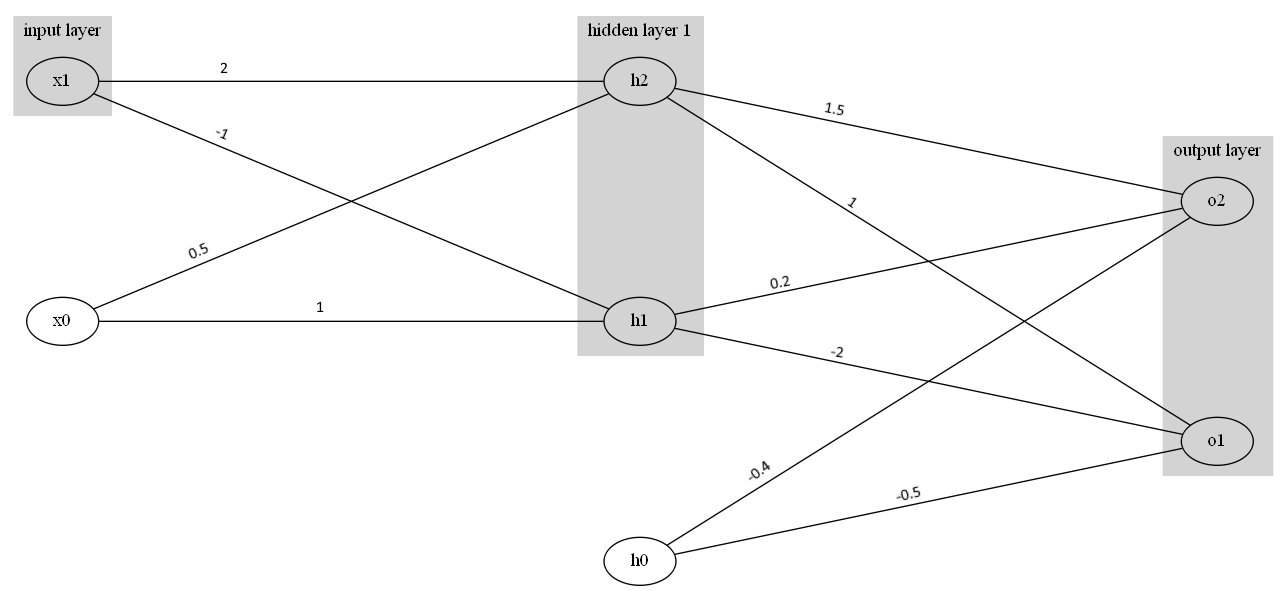
\includegraphics[scale=0.35]{mcq_graph_export}
\end{center}
A:
\begin{enumerate}
   \item $0.002$
   \item $-6$ 
   \item $-2.079$
   \item $0.111$ \textdagger
\end{enumerate}
\end{document}
    
$$
\frac{\partial E}{\partial w_i}(w) = \frac{\partial \frac{1}{2}\sum_{n=1}^N (\sigma(w^\top x_n) - t_n)^2}{\partial w_i}
$$
$$
\frac{\partial E}{\partial w_i}(w) =\sum_{n=1}^N \frac{\partial \frac{1}{2} (\sigma(w^\top x_n) - t_n)^2}{\partial \sigma(w^\top x_n)-t_n} \cdot \frac{\partial \sigma(w^\top x_n)-t_n}{\partial w^\top x_n}\cdot \frac{\partial w^\top x_n}{\partial w_i}
$$
$$
\frac{\partial E}{\partial w_i}(w) =\sum_{n=1}^N (\sigma(w^\top x_n)-t_n) \cdot \sigma(w^\top x_n)(1-\sigma(w^\top x_n)) \cdot x_{n,i}
$$

$$
\frac{A}{B} = \frac{A}{D}\times\frac{D}{C}\times\frac{C}{B}
$$

$$
E(w) = \frac{1}{2}\sum_{n=1}^N (\sigma(w^{(1)}\cdot\sigma({w^{(0)}}^\top x_n)) - t_n)^2
$$
$$
\frac{\partial E}{\partial w^{(1)}}(w) =  \frac{\partial \frac{1}{2}\sum_{n=1}^N(\sigma(w^{(1)}\cdot\sigma({{w^{(0)}}^\top x_n})) - t_n)^2}{\partial w^{(1)}}
$$
$$
\frac{\partial E}{\partial w^{(1)}}(w) = \sum_{n=1}^N \frac{\partial\frac{1}{2}(\sigma(w^{(1)}\cdot\sigma({{w^{(0)}}^\top x_n})) - t_n)^2}{\partial \sigma(w^{(1)}\cdot\sigma({{w^{(0)}}^\top x_n})) - t_n} \cdot \frac{\partial\sigma(w^{(1)}\cdot\sigma({{w^{(0)}}^\top x_n})) - t_n}{w^{(1)}\cdot\sigma({{w^{(0)}}^\top x_n})}\cdot\frac{\partial w^{(1)}\cdot\sigma({{w^{(0)}}^\top x_n})}{\partial w^{(1)}}
$$
$$
\frac{\partial E}{\partial w^{(1)}}(w) = \sum_{n=1}^N (\sigma(w^{(1)}\cdot\sigma({{w^{(0)}}^\top x_n}))-t_n)\cdot \sigma(w^{(1)}\cdot\sigma({{w^{(0)}}^\top x_n}))(1-\sigma(w^{(1)}\cdot\sigma({{w^{(0)}}^\top x_n})))\cdot \sigma({{w^{(0)}}^\top x_n})
$$
set
$$
z_0 = \sigma({{w^{(0)}}^\top x_n})
$$
$$
\frac{\partial E}{\partial w^{(1)}}(w) = \sum_{n=1}^N (\sigma(w^{(1)}\cdot z_0)-t_n)\cdot \sigma(w^{(1)}\cdot z_0)(1-\sigma(w^{(1)}\cdot z_0))\cdot  z_0
$$

--------------------------------------------------

$$
\frac{\partial E}{\partial w^{(0)}_i}(w) = \frac{\partial \frac{1}{2}\sum_{n=1}^N(\sigma(w^{(1)}\cdot\sigma({{w^{(0)}}^\top x_n})) - t_n)^2}{\partial w^{(0)}_i}
$$
$$
\frac{\partial E}{\partial w^{(0)}_i}(w) = \sum_{n=1}^N \frac{\partial\frac{1}{2}(\sigma(w^{(1)}\cdot\sigma({{w^{(0)}}^\top x_n})) - t_n)^2}{\partial \sigma(w^{(1)}\cdot\sigma({{w^{(0)}}^\top x_n})) - t_n} \cdot \frac{\partial\sigma(w^{(1)}\cdot\sigma({{w^{(0)}}^\top x_n})) - t_n}{w^{(1)}\cdot\sigma({{w^{(0)}}^\top x_n})}\cdot\frac{\partial w^{(1)}\cdot\sigma({{w^{(0)}}^\top x_n})}{\partial {w^{(0)}}^\top x_n}\cdot \frac{\partial {w^{(0)}}^\top x_n}{\partial w^{(0)}_i}
$$
$$
\frac{\partial E}{\partial w^{(0)}_i}(w) = \sum_{n=1}^N (\sigma(w^{(1)}\cdot\sigma({{w^{(0)}}^\top x_n}))-t_n)\cdot \sigma(w^{(1)}\cdot\sigma({{w^{(0)}}^\top x_n}))(1-\sigma(w^{(1)}\cdot\sigma({{w^{(0)}}^\top x_n})))\cdot w^{(1)}\sigma({{w^{(0)}}^\top x_n})(1-\sigma({{w^{(0)}}^\top x_n}))\cdot x_{n,i}
$$
$$
\frac{\partial E}{\partial w^{(0)}_i}(w) = \sum_{n=1}^N (\sigma(w^{(1)}\cdot z_0)-t_n)\cdot \sigma(w^{(1)}\cdot z_0)(1-\sigma(w^{(1)}\cdot z_0))\cdot w^{(1)} z_0(1- z_0)\cdot x_{n,i}
$$
$$
\frac{\partial E}{\partial w^{(0)}_i}(w) = 
$$